%splitting 360 degree angle
\documentclass[tikz,border=10pt]{standalone}
\usepackage{tikz}
\usetikzlibrary{angles,quotes,calc} % Add this for angle labels

\begin{document}

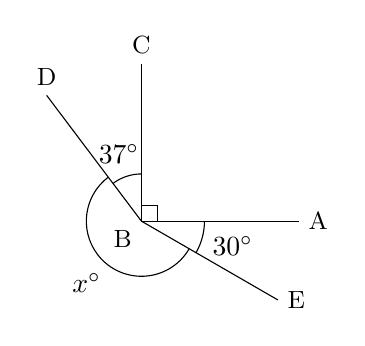
\begin{tikzpicture}[scale=1]
    % Define the points of the cube
    \coordinate (A) at (4,0);
    \coordinate (B) at (2,0);
    \coordinate (C) at (2,2);
    \coordinate (D) at ($(B)+(127:2cm)$); 
    \coordinate (E) at ($(B)+(330:2cm)$); 

    % Draw the visible edges of the cube
    \draw (B) -- (A);
    \draw (B) -- (C);
    \draw (B) -- (D);
    \draw (B) -- (E);

    % Draw the right angle
    \draw (B) ++(0:0.2) -- ++(90:0.2) -- +(180:0.2);
    
    % Draw the angle between lines
    \pic [draw, "$37^{\circ}$", angle eccentricity=1.5, angle radius=0.6cm] {angle = C--B--D};
    \pic [draw, "$x^{\circ}$", angle eccentricity=1.5, angle radius=0.7cm] {angle = D--B--E};
    \pic [draw, "$30^{\circ}$", angle eccentricity=1.5, angle radius=0.8cm] {angle = E--B--A};

    % Place the labels with smaller font size
    \node at (A) [right,font=\small] {A};
    \node at (B) [below left,font=\small] {B};
    \node at (C) [above,font=\small] {C};
    \node at (D) [above,font=\small] {D};
    \node at (E) [right,font=\small] {E};
    
\end{tikzpicture}

\end{document}